\documentclass{article}
\usepackage[utf8]{inputenc}
\usepackage[russian]{babel}
\usepackage{mathtools}
\usepackage{graphicx}

\textwidth=180mm    
\oddsidemargin=-10mm 

\title{Работа 2.4. {\it Определение вязкости воздуха
по скорости течения через тонкие трубки}}
\author{Руденко Ирина и Миллер Сергей, 494}
\date{\today}

\begin{document}

\maketitle
\textbf{Цель работы:}
    \begin{enumerate}
    \item Экспериментально выявить участки ламинарного и турбулентного течения; 
    \item Определить число Рейнольдса; 
    \item Определить вязкость воздуха; 
    \item Экспериментально определить зависимость расхода воздуха в трубках от радиуса.
    \end{enumerate}
\textbf{В работе используются:} металлические трубки, укрепленные на горизонтальной подставке; газовый счетчик; микроманометр типа ММН; стеклянная U-образная трубка; секундомер.

\textbf{Теоретическое введение.}
Если два соприкасающихся слоя жидкости или газа текут с разной скоростью, то между ними возникает сила вязкого трения. Та же сила может действовать на твёрдые тела (по касательной к поверхности), помещённые в поток жидкости или газа. Причина возникновения этой силы заключается в следующем. Скорость частиц в текучей среде складывается из средней скорости потока и хаотической  — тепловой — составляющей. Следовательно, частицы могут перескакивать случайным образом из слоя в слой, перенося вместе с собой часть импульса потока из того слоя, откуда совершен скачок. Перенос же импульса от слоя к слою, согласно 2-му закону Ньютона, эквивалентен силовому взаимодействию между ними. Эта сила направлена по касательной к слоям, поскольку переносится компонента импульса, направленная вдоль среднего потока.Для количественного описания вязкого трения рассмотрим взаимодействие слоёв газа, текущего вдоль оси $x$, скорость потока которого изменяется в поперечном направлении $v_x = v_y(y)$ (см. рис. 1).

Пусть концентрация всюду одинакова и равна $n$, а средняя тепловая скорость хаотичного движения молекул равна$v_T$. Также для дальнейшего рассмотрения нам понадобится понятие длины свободного пробега $\lambda$
— среднего расстояния, которое пролетает молекула между столкновениями с другими молекулами.

Рассмотрим плоскость $y = 0$. Предположим, что через неё сверху вниз пролетают только молекулы, вылетевшие из слоя $0 < y < +\lambda$ (слой 2) и снизу вверх — вылетевшие из слоя $-\lambda < y < 0$ (слой 1). Данное предположение вполне разумно для качественной оценки явления, поскольку молекулы из более дальних слоёв имеют значительно меньшую вероятность добраться до $ y = 0$, поскольку по пути они скорее всего столкнутся с другими молекулами.

\begin{figure}[htp]
\centering
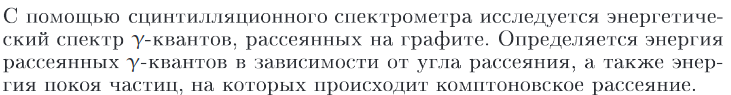
\includegraphics[width=8cm]{1.jpg}
\caption{К выводу оценки коэффициента вязкости}
\end{figure}


Количество молекул, перелетающих из слоя 1 в слой 2 за единицу времени через единичную площадку ({\bold плотность потока}), равно:

\begin{equation}
        j = \frac{dN}{S \cdot dt} = \frac{1}{4} n v_t.
\end{equation}

Каждая из этих молекул массой $m_0$ обладает, помимо хаотично распределённой тепловой составляющей (в среднем $v_T$), дополнительной горизонтальной скоростью, связанной с движением в потоке $v_{1 x} = v_x(-\lambda)$, и горизонтальным импульсом $p_{1 x} = m_0 v_{1 x}$.
И наоборот, из слоя 2 в слой 1 поступает такое же количество молекул, но их средний горизонтальный импульс равен $p_{2 x} = m_0 c_{2 x}$. Горизонтальный импульс, который они переносят в сумме в единицу времени, и есть касательная сила вязкого трения:



$F_x = (\frac{dP_x}{dt})_{2 \to 1}  - (\frac{dP_x}{dt})_{1 \to 2} = j S (p_{2 x} - p_{1 x}) = S \cdot \frac{1}{4} m_0 n v_T \cdot (v_{2 x} - v_{1 x}).$



Считая $\lambda$ достаточно  малой,  раскладываем  по  Тэйлору $v_{2 x} - v_{1 x} = v_{x}(\lambda) - v_{x}(-\lambda)$, из чего получим окончательное
выражение для силы вязкого трения. В общем виде оно выглядит
следующим образом:

\begin{equation}
        F_x = S \eta \frac{d v_x}{dy}, 
\end{equation}

где $\eta$— коэффициент вязкости (сокращенно вязкость), $y$ — направление, перпендикулярное потоку, $S$ — площадь поверхности, для которой рассчитывается приложенная сила. В общих чертах механизм возникновения вязких сил трения во всех текучих средах (жидкостях и газах) одинаков, и формула (2) представляет собой определение
коэффициента вязкости.Для идеального газа, как следует из приведенных выше выкладок, вязкость можно оценить
по порядку величины:

\begin{equation}
        \eta_{Г} \sim \frac{1}{2} m_0 n v_T \lambda = \frac{1}{2} \rho v_t \lambda, 
\end{equation}

Более детальное рассмотрение даёт значение вязкости, отли-
чающееся от полученного на множитель $\frac{2}{3}$. Хотя такое отличие не существенно для оценки по порядку величины, этот ответ является общепринятым для оценки $\eta$:

\begin{equation}
        \eta_{Г} \sim \frac{1}{3} \rho v_t \lambda, 
\end{equation}

\textbf{Течение вязкой жидкости.} Течение жидкости или газа при наличии вязкости описывается уравнением Навье—Стокса, котороe представляет собой 2-й закон Ньютона, записанный для элемента жидкости.

\begin{equation}
        \rho \frac{d \vec{v}}{d t} = - \bigtriangledown P + \eta \cdot \bigtriangleup \vec{v}.
\end{equation}

Слагаемое в левой части есть масса единичного объёма на его ускорение; первое слагаемое в правой части есть градиент давления, дающий нормальную компоненту силы взаимодействия жидких элементов друг с другом; второе же получается именно из силы вязкого трения ($\bigtriangleup$ — оператор Лапласа). Имеется два существенно различных класса течений. Ламинарное течение — течение, происходящее без перемешивания и пульсаций, в параллельных слоях жидкости; турбулентное течение, в котором образуются вихри и пульсации, а слои беспорядочно перемешиваются. Точные решения уравнения Навье—Стокса (5) существуют только для ламинарных течений. В общем же случае, несмотря на кажущуюся простоту (5), динамика жидкости, описываемая им, может быть крайне сложна — проблема аналитического описания (и даже численного расчёта) турбулентности является до сих пор до конца нерешенной и актуальной научной задачей.


То, каким будет данное конкретное течение, зависит от соотношения физических параметров, входящих в уравнение (5), и от геометрических характеристик системы. Если у системы есть характерный размер $r$ (радиус трубки при течении по трубе, радиус шарика при обтекании его внешним потоком и т. п.), то из $r$, плотности, вязкости $\eta$ и характерной скорости потока $v$ можно составить безразмерное соотношение:

\begin{equation}
        Re = \frac{\rho v r}{\eta}
\end{equation}
 
называемое числом Рейнольдса.
Безразмерные параметры отражают связь между физическими явлениями, происходящими на разных масштабах, и часто ис-
пользуются при описании сложных физических явлений, для которых нет точных решений. Величины $v, \rho, r, \eta$ могут меняться в широком диапазоне (например, течение воздуха в аэродинамической трубе диаметром в десятки метров и течение воды в капилляре), но если число $Re$ для этих случаев будет одинаково, то эти течения будут подобны друг другу. Такие зависимости в физике называют законами подобия.

Число Рейнольдса характеризует (по порядку величины) отношение кинетической энергии элемента жидкости к работе сил вязкого трения, совершаемой над ним. Действительно, кинетическая энергия в кубике со стороной $r$ равна
$ k \sim \frac{\rho r^3 v^2}{2}$, сила трения $F \sim \frac{r^2 \eta v}{r}$ и её работа $ A_F \sim F r \sim \eta v r^2 $, откуда

\begin{center}
    $Re \sim \frac{K}{A_F}$.
\end{center}

Вязкие силы стремятся стабилизировать течение, тогда как избыток кинетической энергии может приводить к переходу её части в вихревое движение. Таким образом, можно заключить, что большие числа Рейнольдса благоприятствуют рождению турбулентных течений, а при малых Re течение будет, скорее всего, ламинарным.

Эксперимент подтверждает эти рассуждения: для заданной геометрии течения существует критическое значение числа Рейнольдса $Re_{кр}$, так что при $Re > Re_{кр}$ ламинарное течение оказывается неустойчивым и рождается турбулентность. Для течения по трубе эксперимент даёт $Re_{кр}\sim 10^3.$

\textbf{Течение по трубе.} Рассмотрим стационарное течение вязкой жидкости или газа по трубке круглого сечения радиуса $R$. Получим выражение для скорости потока в зависимости от расстояния до центра трубы $r$. При малых скоростях течение будет ламинарным и стационарным, поэтому $ dv/dt = 0$. Кроме того, в трубе постоянного сечения не может зависеть от $x$, поскольку через каждое сечение должно проходить одинаковое количество жидкости, следовательно, скорость можно считать зависящей только от $r: v = v(r)$, давление же при этом зависит только от координаты вдоль трубы. Тогда, воспользовавшись известным выражением для оператора Лапласа в цилиндрических координатах, получим из уравнения (5) следующее:

\begin{equation}
        \frac{dP}{dx} = \eta \frac{1}{r} \frac{d}{d r} (\frac{1}{r} \frac{dv}{dr})
\end{equation}

К этому необходимо добавить граничное условие на $v(r)$: скорость течения на поверхности трубы должна быть нулевой (условие прилипания), $v(R) = 0$. Левая часть уравнения (7) не зависит от $r$, поэтому дважды проинтегрировав его по $r$ с учётом граничного условия получим

\begin{center}
    $ v = - \frac{dP}{dx} \frac{1}{4 \eta} (R^2 - r^2). $
\end{center}


С учётом того, что и $dP/dx = const$ (т. е. $P(x)$— линейная функция), получим окончательно

\begin{equation}
        v = \frac{P_1 - P_2}{L} \frac{1}{4 \eta} (R^2 - r^2),
\end{equation}

где $P_2$ и $P_1$ — давления на концах трубы, а $L$ — длина трубы

\begin{figure}[htp]
\centering
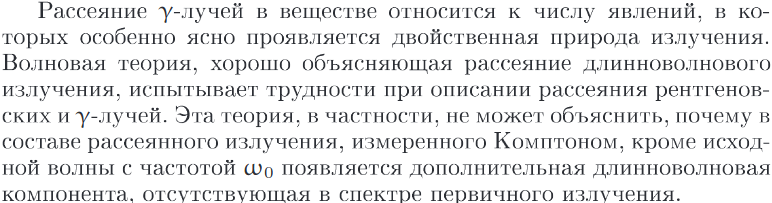
\includegraphics[width=9cm]{2.jpg}
\end{figure}


\begin{figure}[htp]
\centering
\includegraphics[width=14cm]{0ex.png}
\end{figure}


\begin{figure}[htp]
\centering
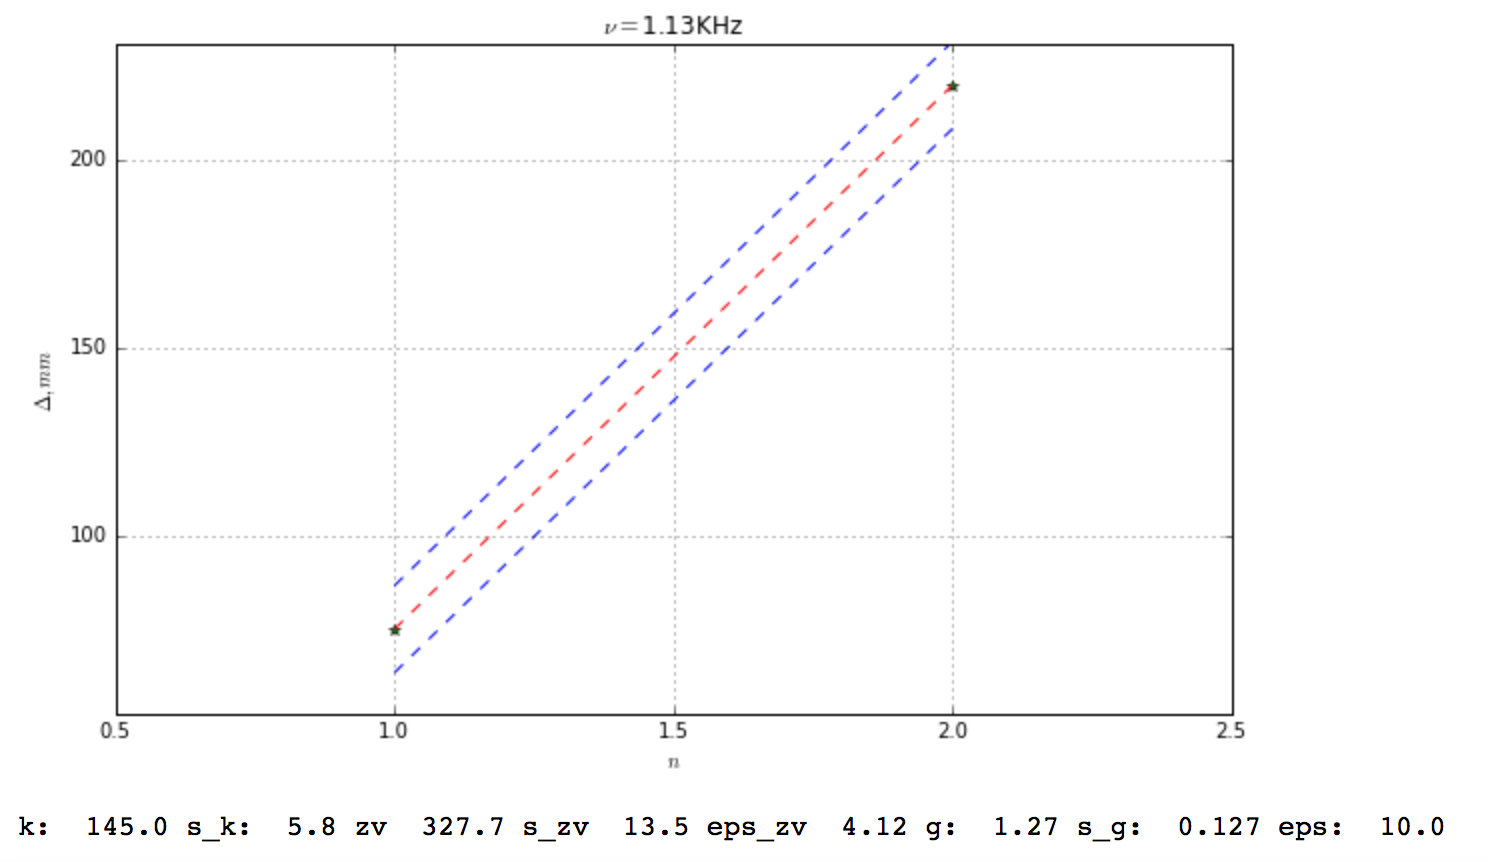
\includegraphics[width=10cm]{1ex.png}
\end{figure}


\begin{figure}[htp]
\centering
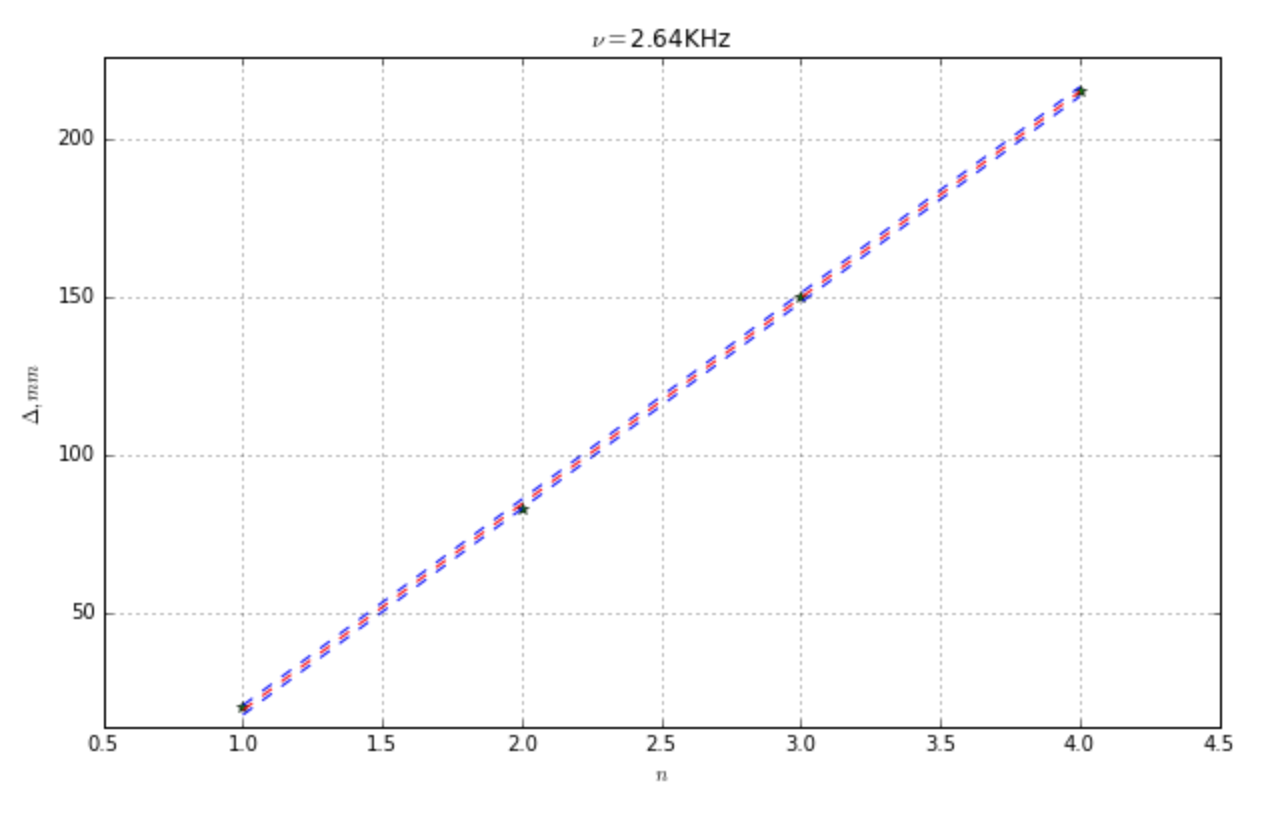
\includegraphics[width=9cm]{2ex.png}
\end{figure}


\newpage
\textbf{Ход работы:}

\begin{enumerate}

    \item  Будем измерять вязкость воздуха, снимая зависимость разности давлений $\bigtriangleup P$ на некотором участке трубы от расхода воздуха $\bigtriangleup Q = \frac{\bigtriangleup V}{\bigtriangleup t}$, при этом $\bigtriangleup V$ измеряется газовым счетчиком, а $\bigtriangleup t$— секундомером. Измерения будем проводить на участке с установившимся потоком (для трубки с диаметром 3.85мм и 5.25 возьмём участок длиной 50 см).Множитель на стойке микроманометра возьмём равным 0,2. Постепенно увеличим расход, начиная с маленьких перепадов давления.
    
   Будем вычислять $\mu$ из формулы Пуазейля(10).
    
    \begin{equation}
        \mu = \frac {\pi R ^ 4 \Delta P}{8 QL}
      \end{equation}
    
    Оценку $Re$ получим из следующих соотношений:

    \begin{equation}    
        Re = \frac{\rho vr}{\nu} = \frac{\rho lrS}{\nu tS} = \frac{\rho Q}{\nu \pi r}
    \end{equation}
        
    Погрешность $\sigma_\mu$ определим из формулы для погрешности функции многих переменных:

    \begin{equation}
        \bigg(\frac{\sigma_\mu}{\mu}\bigg) ^ 2 =    4^2 \bigg(\frac{\sigma_r}{r}\bigg) ^ 2 +  \bigg(\frac{\sigma_{\Delta P}}{\Delta_{min} P}\bigg) ^ 2 + \bigg(\frac{\sigma_L}{L}\bigg) ^ 2 +
        \bigg(\frac{\sigma_Q}{Q}\bigg) ^ 2 
    \end{equation}
    
    
    При измерениях:

        $\sigma_L = 0.5 см$, $\sigma_r = 0.05 мм$, $ \sigma_P = 1 $ деление (или 0.2 * 9.8 Па), для $Q = \frac{V}{\Delta t}$ можно считать, что V измеренно точно, так как кратное число делений с большой вероятностью попадет в зазор $t \pm \sigma_t$, где $\sigma+t = 0.5$ c.
    
    
    \item График зависимости $\Delta P$ от расхода воздуха для трубки диаметром 3.85см
    
    \begin{center} 
        \includegraphics[width=10cm]{g1.png}
    \end{center}
    
    
    
    $\mu = 1.68 \cdot 10^{-5}$  $\sigma_{\mu}: = 10^{-6}$  $\varepsilon_{\mu} = 6.0$ 
   

    $Re \sim  1115$
    
    
    \item График зависимости $\Delta P$ от расхода воздуха для трубки диаметром 5.25см
     
    \begin{center}
    \includegraphics[width=10cm]{g2.png}
    \end{center}
    
    
    $\mu = 1.79 \cdot 10^{-5}$  $\sigma_{\mu}: = 8 \cdot 10^{-7}$  $\varepsilon_{\mu} = 4.0$ 
    
    $Re \sim  995$
    
    \item График зависимости $\Delta P$ от расхода воздуха для трубки диаметром 3.85см на заведомо турбулентном участке (начальный участок, искривление)
     
    \begin{center}
    \includegraphics[width=10cm]{g3.png}
    \end{center}
    
    
    $\mu = 2.08 \cdot 10^{-5}$  $\sigma_{\mu}: = 9 \cdot 10^{-7}$  $\varepsilon_{\mu} = 4.0$ 
    
    $Re \sim  838$
    
     \item В итоге получаем экспериментальные значения для $\mu$ в зонах ламинарного течения, и одно значение при турбулентном(на трубе $d = 5.25$ мм):
     
     $\mu_{\text{ex lam 3.85}} = (1.68 \pm 0.10) \cdot 10^{-5} \text{Па с}$
     
    $\mu_{\text{ex lam 5.25}} = (1.79 \pm 0.08) \cdot 10^{-5} \text{Па с}$
          
    $\mu_{\text{ex turb 5.25}} = (2.08 \pm 0.09) \cdot 10^{-5} \text{Па с}$
     
     Теоретическая вязкость при $\lambda \sim 10^{-5}$: 
        \begin{equation}
                \mu_{th} = \frac{1}{3} \rho v_T \lambda = \frac{1}{3} \rho \lambda \sqrt{\frac{3RT}{m_{mol}}} \approx  2.02 \cdot 10^{-5} \text{Па с}
        \end{equation}
        где $m_{mol}$ - молярная масса воздуха
        
    Также в таблицах можно найти значение вязкости воздуха для $T \sim 15 - 20^o C:$
    
    $\mu_{table} = 1.78 \cdot 10^{-5} \text{Па с}$
     
     
    \item Зависимость P от длины для трубок диаметром 3.85см и 5.25см при малом давлении
        \begin{center}
        \includegraphics[width=7cm]{p1.png}
        \end{center}
        

        \begin{center}
        \includegraphics[width=7cm]{p2.png}
        \end{center}
        
        Заметим, что при малом давлении участки турбулентности отсутствуют на графиках
    
    
    \item Зависимость P от длины для трубкок диаметром 3.85см и 5.25см при увеличении давления
        \begin{center}
        \includegraphics[width=7cm]{p3.png}
        \end{center}
        
        \begin{center}
        \includegraphics[width=7cm]{p4.png}
        \end{center}
        
        При увеличении давления график качественно изменился в результате проявления участков турбулентности на начальном отрезке трубки    
\end{enumerate}

 \pagebreak
    \begin{center}
    \includegraphics[width=13cm]{data.png}
    \end{center}
        
        
\end{document}


